\documentclass{article}
\usepackage{graphicx}
\usepackage{fvextra}
\usepackage{hyperref}
\usepackage{geometry}
 \geometry{
    a4paper,
    total={170mm,257mm},
    left=20mm,
    top=20mm,
}
\hypersetup{
    colorlinks=true,
    urlcolor=blue,
}

\title{David's Universal Number Kounter}
\author{David Farrell}
\date{May 2025}

\begin{document}

\maketitle

\section{Introduction}

David's Universal Number Kounter, "dunk", is a fully-16-bit microcoded CPU designed in Logisim-evolution. Let me explain those terms. First, fully-16-bit: everything in dunk has a 16-bit bit width. The registers, buses, instructions, and even memory cells in dunk are 16 bits in width. Memory is addressed in 16 bit words, rather than bytes; each memory address (themselves 16 bits) refers to a 16 bit word in main memory, and read and write operations only deal with these 16-bit words. This is for simplicity; this project was created as an educational exercise, at a time where my knowledge of computer architecture was... limited. By \textit{microcoded} I mean that every machine code instructions is translated on-the-fly by the control unit into a sequence of so-called ``micro-code instructions'' which instruct the various parts of the CPU on how to actually carry out the instructions. While a machine code instruction might be something like, "load the value of memory at the address stored in register 1 into register 2", micro-code instructions are much more granular; for instance, the aforementioned instruction would be carried out by the sequence "output the value of register 1 to the address bus; send the output of the memory unit to the data bus; write the content of teh data bus to register 2". As for logisim-evolution; \href{https://cburch.com/logisim/docs/2.0b17/index.html}{Logisim} is (was) ``an educational tool for designing and simulating digital logic circuits'' created in 2005 by Google software engineer Dr. Carl Burch. It is a schematic-based editor, and is (was) used widely as a learning tool\footnote{I encountered it in Physics140 at the University of Auckland during my undergrad, though I had used it several years beforehand}. Unfortunately, active development of Logisim was discontinued by Burch in 2011. Fortunately, Logisim is open source, and the torch was picked up by the open source community, who maintain a fork, Logisim-evolution, which sees active development to this day. Hereafter I'll drop the "-evolution" and refer to Logisim-evolution simply as "logisim", for brevity's sake. Now, a brief (optional) tangent on the context in which this project was created.

\subsection{Context}

When I was quite young - mid-to-late teens - as a hobbyist C/C++ programmer of several years and general computer enthusiast, I was shocked to learn that it was possible to build a functioning computer in Minecraft (of all things). My curiosity piqued, I of course went about learning how this was done. This led me to learn all about digital logic; logic gates and multiplexors and flip-flops and what-not. I absolutely adored the topic, and went on to have great fun making components such as adders and registers first in Minecraft and then Logisim. I'd long wanted to implement my own fully-functioning CPU, however, I never quite had the knowledge to put all the pieces together. In particular, I couldn't envision how a \textit{control unit}, the unit which actually instructs a CPU to carry out the instructions fed to it, could be created\footnote{Of course, this is not how \textit{all} CPUs work; many, especially more modern, CPUs are organised into more of a ``pipeline'' structure, where it doesn't take so much centralised control for the units to know what to do with an instruction. But I didn't know this yet.}. My interests turned elsewhere, and I never ended up completing the task. That was, until, in early 2025 my partner was watching a Youtube video of someone demonstrating a CPU \textit{they'd} built in logisim, and I was half-listening while carrying out some household chore. I heard them explain that their control unit uses micro-codes, and immediately I knew how to complete my long-dormant ambition. My interest in it was instantly reignited, and I proceeded to spend a month glued to logisim working on it (even through my two-week holiday to New Zealand, and catching COVID while there). This didn't leave much time for learning of the industry-standard solutions to the many problems I encountered along the way, and so the design diverges in some ways from the typical, but - most importantly - it works! And I learned a lot. What's more, since logisim includes the ability to load binary files into its RAM and ROM components, I've also written an assembler for it, so it can be programmed from a common text editor.

\newpage
\subsection{Why is it called that?}

During the design process, I jokingly named the program counter register the ``program kounter''. This is in homage to a 2021 \href{https://x.com/6thgrade4ever/status/1433519577892327424}{tweet} by twitter user @6thgradeforever:

    \begin{center}
\includegraphics[width=0.75\textwidth]{images/runk.png}\end{center}

This is reflected in the .circ file, and the assembler; the program counter is always refered to as the program kounter, and ``pk" addresses the register in the assembly language. When it came time to actually put a name to this project, naturally I named it ``\textit{David's} universal number kounter", since, being a turing machine, it is quite literally a universal number counter. Now, this is not to imply that I consider myself among ``the most consequential figures in the tech world''; in fact, the whole time - up until it came time to source an image to insert into this pdf - 	I actually thought I was referring to the alt-text on \href{https://xkcd.com/2347/}{xkcd 2347},

    \begin{center}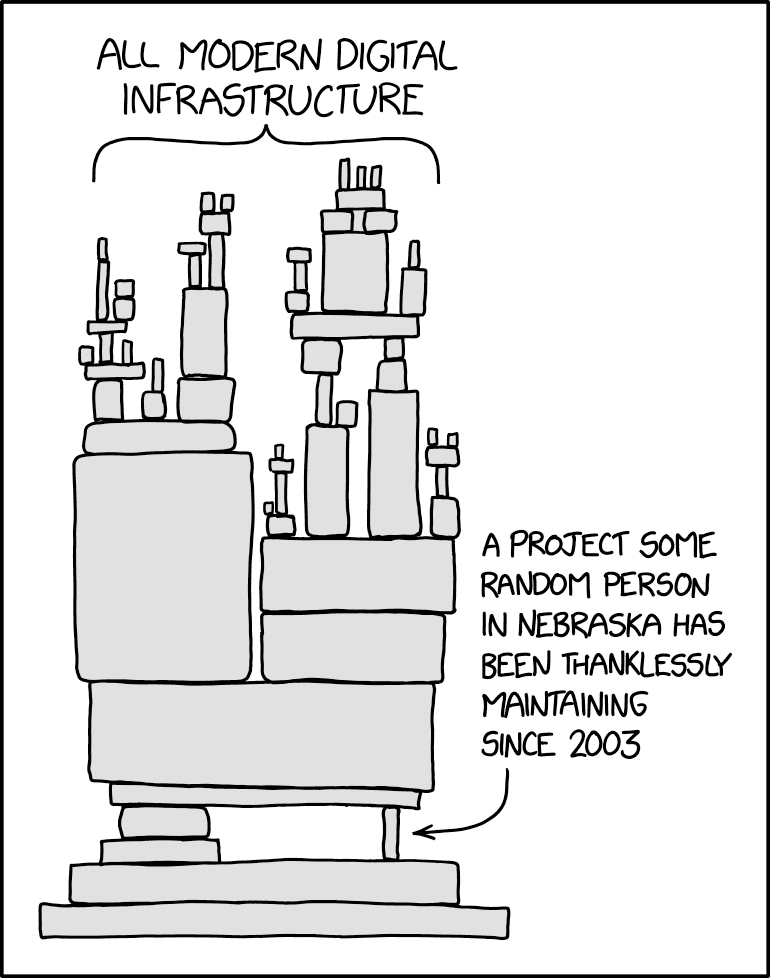
\includegraphics[width=0.5\textwidth]{images/2347.png}\end{center}

which does \textit{not} contain the phrase ``the most consequential figures in the tech world''. As it turns out, however, it \textit{also} doesn't contain the phrase ``ronald's universal number kounter'', which instead comes from @6thgradeforever's tweet.

\section{Quick Start: Getting Something To Happen}

Dunk can be viewed by opening the ``dunk.circ'' file in logisim. There you can see the various components, and connections between them. The ``poke'' tool in logisim can be used to examine the components, and see the values carried on wires, and so on. The quickest way to get something to happen is to load one of the example binaries from the folder ``examples/bin'' into memory and turn on auto-tick. To do this, right-click on the RAM unit (lower right) and select ``Load Image...'';

    \begin{center}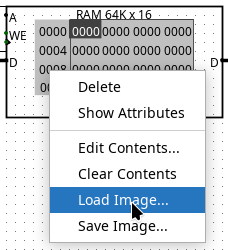
\includegraphics[width=0.25\textwidth]{images/load_image.png}\end{center}

Then navigate to and select the file. You should then be greeted by a dialog box like this.

    \begin{center}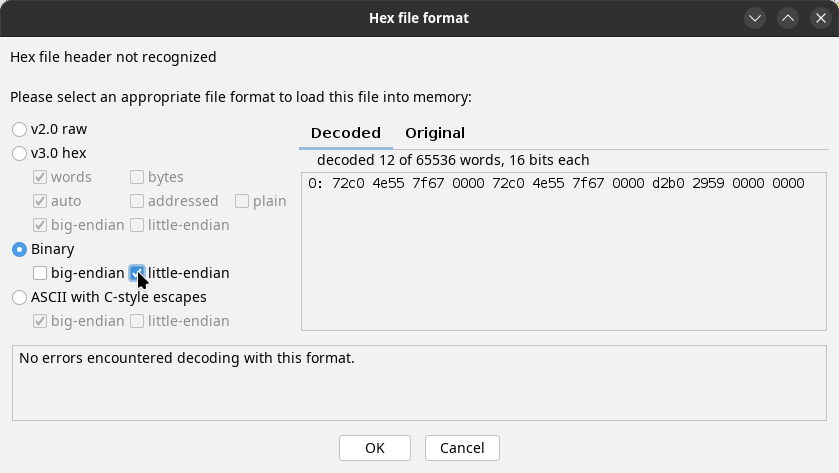
\includegraphics[width=0.5\textwidth]{images/little_endian.png}\end{center}

Then, and this is important -
    \begin{center}{\color{red} YOU MUST SELECT ``LITTLE-ENDIAN'' OR IT WILL NOT WORK}\end{center}
Unfortunately, there is no setting (that I know of) to make logisim \textit{default} to little endian, so you have to click it every time, which is annoying. Having done this, click "OK". You can then begin the clock ticking by the hotkey ``Ctrl+k'', or selecting ``Auto-Tick Enabled'' under the ``Simulate'' menu. The simulation should then begin, and the CPU will run the code. The speed of Auto-Tick can be changed under the ``Simulate'' menu; I recommend cranking it up. So, go ahead, run the \Verb|hello world| example. See what happens. I'm sure you'll be surprised.

\section{The Instruction Set And Assembler}

Dunk uses an instruction set of my own design. It doesn't have any innovative features; remember, this project was really just to see if I could. The instruction set shares some similarities with the x86 instruction set, although I wouldn't say it is ``based'' on it. Associated with dunk is the assembler ``dunkasm'', which compiles dunk assembly files into runnable machine code binary files. The instruction set itself is documented in the file ``instruction set.pdf'' which, at the time of writing, requires updating. Its current state is also ``documented'' in the source code for dunkasm.

The assembly language features some quality-of-life improvements over the typical assembly language, to the point where it doesn't actually \textit{look} very much like the typical assembly language. A fairly immediate example of this is the \textit{human-readability} of instructions. For instance, in place of something like ``\Verb|bgez|'', as in the RISC-V instruction set RV32I, I named my analogue ``\Verb{goto_if_nonnegative}''. The reason for this choice is that I simply don't believe there's any valor in unnecessary suffering. I simply don't see why someone writing assembly can't have a nice time doing it, and human-readability of instructions significantly reduces the amount of unnecessary suffering involved.

Another quality-of-life feature included in the assembler is \textit{aliases}. The commands ``alias'' and ``dealias'' allow one to define and undefine aliases; for instance, the command \Verb|alias x r0| defines an alias ``\Verb|x|'', instances of which the assembler will replace with the string ``r0''. Instructions, registers, memory addressse and constants can all be given aliases. The specific behaviour of syntax rules for aliases will be detailed in the assembly manual. Additionally, the assembler has inbuilt aliases, such as, for instance, the alises ``argument1''-``argument9'', where \Verb|argumentN|, for \Verb|N| from 1-9, is replaced by \Verb|*(sr1+N)|, which is a reference to the $N$th word on the stack preceeding the stack pointer \Verb|sr1|.\footnote{Which itself can be accessed via the alias \Verb|sp|} This can be used inside a function to refer directly to the arguments, which are pushed onto the stack, in reverse order, before a function call. To see this all in action, consider the following code snippet:

\begin{BVerbatim}


    alias x r0
    alias y r1

    remainder:
        set x argument1
        set y argument2
        
        remainder_loop:
	        subtract x y
	        
	        goto_if_negative x remainder_done
	        
	        goto remainder_loop
        
        remainder_done:
	        add x y
	        set result x
	        return
	        
	        
\end{BVerbatim}

This code defines a function which copies the two arguments into registers, computes the remainder of \Verb|argument1| on division by \Verb|remainder2|, and returns the result\footnote{Of course, it doesn't account for the possibility of negative inputs. A more robust version is provided in the examples folder.}. The return is achieved via last two lines. The line \Verb|set result x| uses the inbuilt \Verb|result| alias, which is replaced by the assembler with \Verb|*(sr1+1)|, which points to the first word on the stack preceding the stack pointer. The following code snippet calls this function on the arguments 17 and 7 and stores the result in the register \Verb|r0|.

\begin{center}
\begin{BVerbatim}
push 7
push 17

call remainder

pop r0
pop
\end{BVerbatim}
\end{center}

Note the two pops. The first pop saves the return value of the function into \Verb|r0| and increments the stack pointer (the stack grows downwards), while the second has no argument, and simply increments the stack pointer, popping off the now-unnecessary 7. While they are both written ``pop'', on a machine level, these are entirely distinct instructions. This illustrates the third quality-of-life feature in dunkasm; the same name can refer to different instructions. The assembler examines the number and type of arguments provided to an instruction, and selects the specific instruction corresponding to the name provided given but also the arguments provided. The main instance of this is the \Verb|set| command. You may also have noticed the lines \Verb|set x argument 1| and \Verb|set result x|. The first loads a word from memory into a register, while the second saves a word from a register into memory. Not only does \Verb|set| handle these two cases, in fact \Verb|set| can be compiled down to any one of (at the time of writing) \textit{fifty six} different machine code instructions, corresponding to all possible cases of ``set''ing some register or memory equal to some other thing by copying the value from one into the other.

\end{document}
